\chapter{S.I.D.E. - Architecture}
Il sistema S.I.D.E. (SCADA Intrusion Detection Environment) è strutturato in moduli indipendenti ma interconnessi, ciascuno responsabile di una parte specifica del flusso di raccolta, analisi e visualizzazione dei dati.  
L’obiettivo principale è la rilevazione di anomalie e attacchi in ambienti SCADA, attraverso un’architettura a microservizi basata su messaggistica, analisi di pacchetti e modellazione comportamentale.

\section{Architettura Generale}
L’architettura complessiva si articola nei seguenti componenti principali:
\begin{itemize}
    \item \textbf{side-sniff}: modulo di sniffing e analisi del traffico SCADA;
    \item \textbf{side-device-discovery}: servizio di scoperta e registrazione dei dispositivi in Neo4j;
    \item \textbf{side-api-back-end}: API REST per l’interazione tra backend, database e frontend;
    \item \textbf{side-frontend}: interfaccia grafica per la visualizzazione e il monitoraggio realtime;
    \item \textbf{side-ml-models}: componente di machine learning integrato nello sniffer;
    \item \textbf{Device Simulators}: insieme di dispositivi SCADA simulati (Modbus, OPC-UA, Snap7).
\end{itemize}

%%% Side-Sniff
\section{side-sniff}
Il modulo \texttt{side-sniff} rappresenta il core del sistema: un \textit{IDS} modulare e cross-platform per la cattura, l'analisi e la classificazione del traffico SCADA/ICS.  
Il design è pensato per essere leggero in fase di cattura ma estendibile nelle componenti di analisi, con particolare attenzione a prestazioni, robustezza e facilità di estensione per nuovi protocolli.

\subsection{Obiettivi funzionali}
\begin{itemize}
  \item Cattura passiva del traffico su interfacce di rete (Linux, Windows, macOS).
  \item Parsificazione multilivello (IP, Trasporto) con dissector specifici per Modbus, OPC-UA, Snap7.
  \item Rilevamento multi-livello: firme (rule matching), rilevamento statistico (Z-scoring) e apprendimento automatico (classificazione/anomalia).
  \item Pubblicazione dei vari messaggi di alert mediante protocollo MQTT per tipologia di Protocollo gestito.
\end{itemize}

\subsection{Panoramica dello Sniffer}
Il servizio opera come \textit{daemon/service} e si compone di tre blocchi principali:
\begin{enumerate}
  \item \textbf{Capture layer}: gestisce la cattura del traffico di rete attraverso librerie compatibili con \texttt{libpcap} / \texttt{Npcap}, utilizzate internamente da \texttt{Scapy}. È responsabile dell’acquisizione dei pacchetti e dell’applicazione di eventuali filtri BPF per limitare il traffico analizzato.
  \item \textbf{Dispatcher}: riceve i pacchetti grezzi catturati, effettua il parsing dei layer di rete e trasporto (IP, TCP/UDP) e identifica il protocollo SCADA/ICS associato tramite la \textit{protocol tree}.
  \item \textbf{Handler}: contiene i parser specifici per i protocolli industriali supportati (Modbus, Snap7, OPC-UA) e i moduli di analisi e rilevamento (rule-based, statistico, o basato su machine learning).
\end{enumerate}

\subsection{Procedura operativa (step-by-step)}
La seguente sequenza descrive il flusso operativo interno del modulo \texttt{side-sniff}, coerente con l’implementazione attuale del prototipo Python.

\begin{enumerate}
  \item \textbf{Avvio e scelta dell'interfaccia:} all'avvio, il programma può essere eseguito in modalità \textit{interactive} (CLI/TUI) oppure come \textit{daemon}, con l'interfaccia già specificata nel file di configurazione.  
  In modalità interattiva, l’utente seleziona l’interfaccia di rete su cui effettuare la cattura, tramite la funzione \texttt{select\_interface()} che interroga le API di sistema fornite da \texttt{libpcap/Npcap} (via \texttt{Scapy}).  
  La selezione può includere un filtro BPF opzionale, che verrà applicato durante la cattura per ridurre il traffico non rilevante.

  \begin{figure}[!ht]
    \centering
    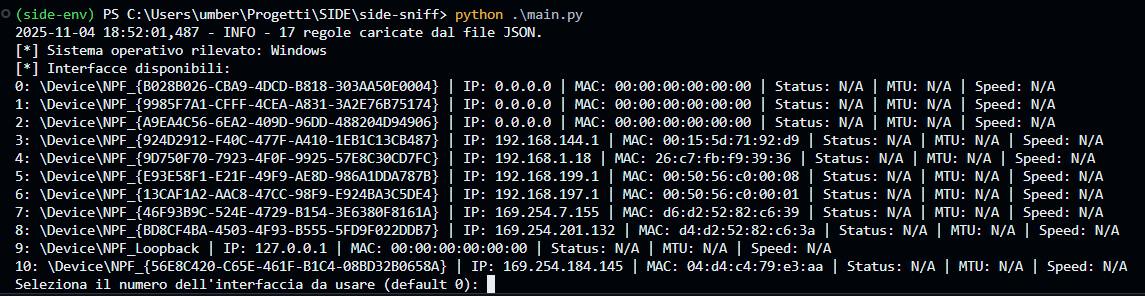
\includegraphics[width=0.75\textwidth]{img/side-sniff-image/select_interface.png}
    \caption{Schermata di selezione dell’interfaccia in \texttt{side-sniff}}
    \label{fig:interface_selection}
  \end{figure}

  \item \textbf{Inizializzazione del Capture layer:} una volta scelta l’interfaccia, il modulo \texttt{core.side\_sniffer\_core} avvia un thread dedicato alla cattura tramite la funzione \texttt{run\_sniffer\_in\_thread()}.  
  Tale funzione utilizza \texttt{scapy.sniff()} per aprire la sessione di cattura, specificando:
  \begin{itemize}
    \item l’interfaccia selezionata (\texttt{iface});
    \item la funzione di callback \texttt{dispatch\_packet} per l’elaborazione di ogni pacchetto;
    \item l’eventuale filtro BPF (al momento lasciato vuoto nel prototipo);
    \item una funzione di terminazione che consente di arrestare lo sniffer in modo controllato tramite segnale \texttt{KeyboardInterrupt}.
  \end{itemize}

  \item \textbf{Acquisizione e dispatch dei pacchetti:} i pacchetti grezzi acquisiti vengono passati direttamente al \textit{Dispatcher} attraverso la callback \texttt{dispatch\_packet()}.  
  Quest’ultimo effettua il parsing dei layer di trasporto (\texttt{TCP}/\texttt{UDP}), identifica la porta sorgente o destinazione e consulta la struttura \texttt{protocol\_tree} per associare il pacchetto a un protocollo noto.  
  In caso di corrispondenza, il pacchetto viene inoltrato al rispettivo \textit{handler} (es. \texttt{modbus\_packet\_handler()}, \texttt{s7\_packet\_handler()}, \texttt{opcua\_packet\_handler()}), che si occupa della successiva fase di analisi.

  \item \textbf{Identificazione tramite Protocol Tree:} la componente \texttt{protocol\_tree} costituisce la logica di identificazione dei protocolli SCADA/ICS all’interno dello sniffer.  
  Tale struttura dati è implementata mediante una \textit{Radix Tree} (o \textit{Patricia Trie}), progettata per eseguire ricerche efficienti su chiavi testuali compatte come \texttt{"TCP-502"} o \texttt{"UDP-4840"}, che rappresentano le coppie \textit{layer–porta}.  

  \begin{figure}[!ht]
    \centering
    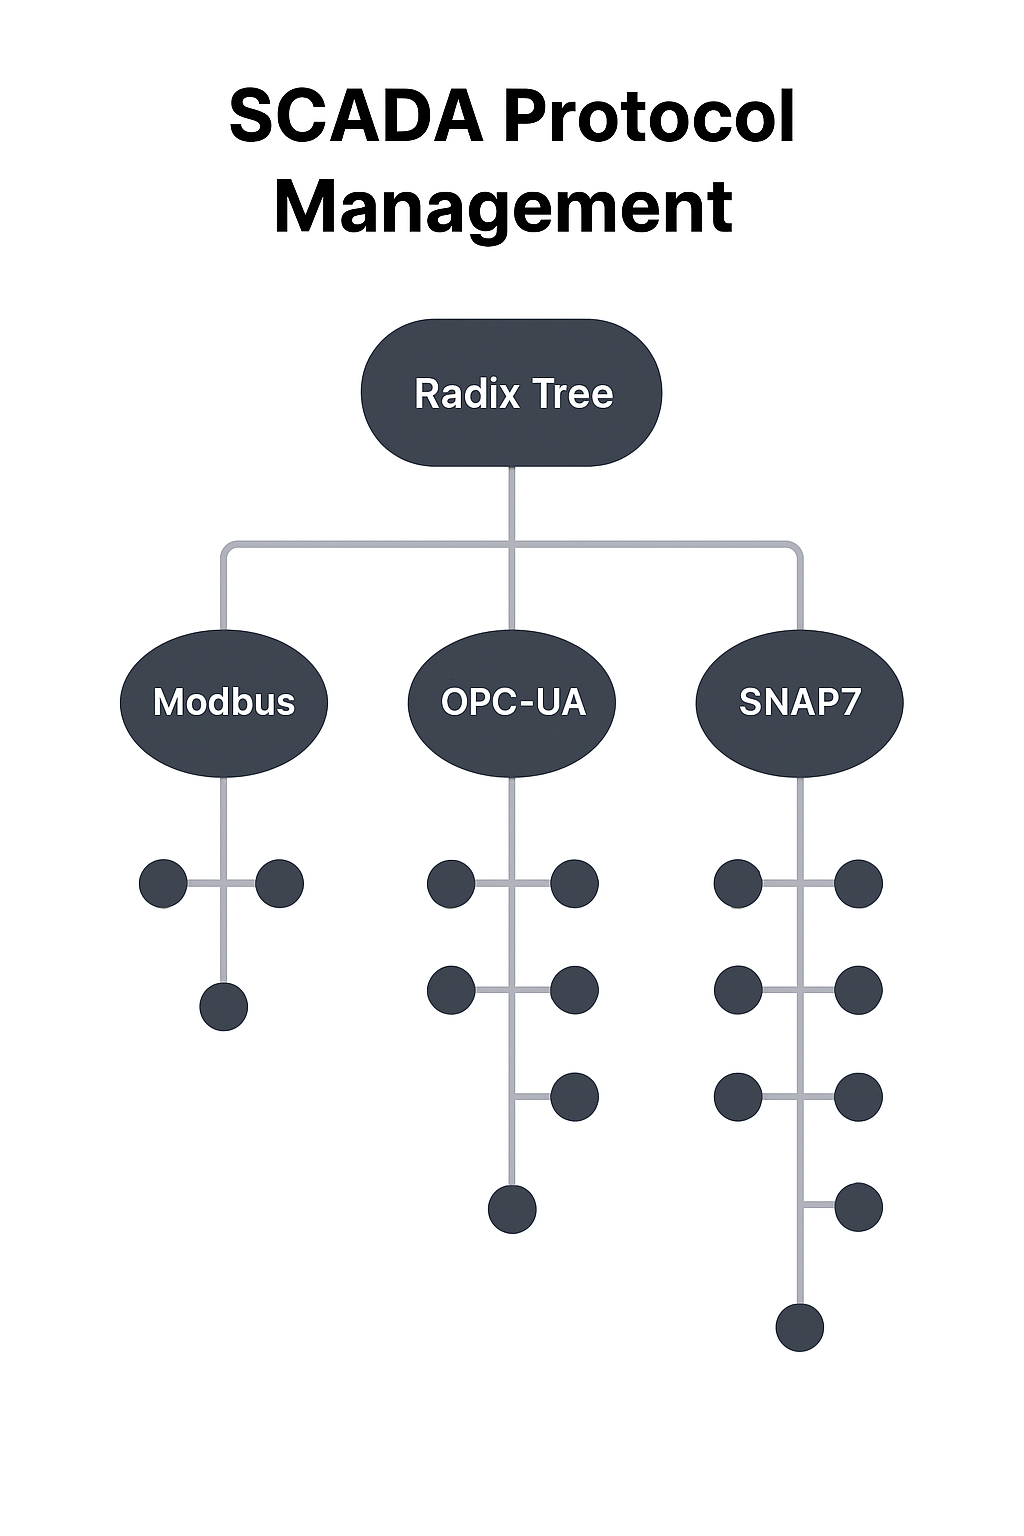
\includegraphics[width=0.5\textwidth]{img/side-sniff-image/radix_tree_protocol.png}
    \caption{Struttura concettuale della \textit{Protocol Radix Tree} di \texttt{side-sniff}}
    \label{fig:protocol_tree_structure}
  \end{figure}

  Durante l’inizializzazione, il modulo \texttt{core.side\_sniffer\_protocol\_tree} importa la classe \texttt{RadixTreeProtocolFilter}, la quale:
  \begin{itemize}
    \item costruisce la Radix Tree popolandola con regole caricate da un file JSON esterno (\texttt{rules.json});
    \item associa a ciascun nodo terminale un insieme di regole che definiscono un protocollo (es. Modbus, S7, OPC-UA);
    \item consente ricerche rapide basate su chiavi di layer e porta, restituendo le regole o i metadati associati al protocollo.
  \end{itemize}

  Il caricamento delle regole avviene tramite la funzione:
  \begin{verbatim}
  protocol_tree.load_from_json(f"{BASE_DIR_RULES}/{RULES_FILE}")
  \end{verbatim}
  dove il file JSON descrive in forma compatta le associazioni tra layer, porta e protocollo:
\begin{lstlisting}[language=python, caption={Formulazione delle regole generali in JSON - SCADA}]
  [
    { "layer": "TCP", "port": 502, "protocol": "Modbus" },
    { "layer": "TCP", "port": 102, "protocol": "S7" },
    { "layer": "TCP", "port": 4840, "protocol": "OPC-UA" }
  ]
  \end{lstlisting}

  In fase di analisi, la funzione \texttt{dispatch\_packet()} costruisce una chiave \texttt{"<layer>-<porta>"} e invoca:
  \begin{verbatim}
  match = protocol_tree.search(key)
  \end{verbatim}
  Se viene trovata una corrispondenza, il protocollo viene riconosciuto e il pacchetto è inoltrato all’\textit{handler} specifico.  

    \item \textbf{Parsing e gestione dei protocolli SCADA:} una volta che il Dispatcher riceve i pacchetti raw dal livello di cattura, essi vengono indirizzati ai moduli \textit{Handler} appropriati, ciascuno specializzato nell’analisi di un protocollo specifico (Modbus/TCP, S7, OPC-UA).  
  Ogni handler esegue il parsing del payload, estrae campi significativi per il livello applicativo e applica controlli di validità e rilevamento anomalie basati su modelli statistici e di \textit{machine learning}.  

  \paragraph{Handler Modbus/TCP}
  Il modulo \texttt{modbus\_packet\_handler} è responsabile dell’elaborazione dei pacchetti TCP diretti alla porta 502.  
  Dopo la verifica dei layer IP e TCP, l’handler estrae il payload grezzo (\texttt{Raw}) e lo passa alla funzione di decodifica \texttt{parse\_modbus\_payload()}, che interpreta la struttura MBAP (Transaction ID, Protocol ID, Length, Unit ID) e la Function Code.  
  In caso di eccezione, viene generato un log diagnostico e registrato l’evento.  
  Ogni pacchetto viene poi convertito in un vettore di \textit{feature} (Function Code, lunghezza del campo dati, presenza di eccezioni) e analizzato dal servizio \texttt{ZScoreService}.  
  Se viene rilevata un’anomalia statistica, il controllo passa al modello ML \texttt{IsolationForestModbusService}, che conferma o smentisce la natura anomala del pacchetto.  
  Gli eventi anomali vengono pubblicati nel sistema di monitoraggio con metadati completi (IP sorgente/destinazione, Function Code, nome funzione, dati in esadecimale).  

  \begin{figure}[!h]
    \centering
    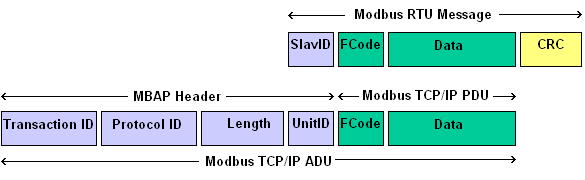
\includegraphics[width=0.85\textwidth]{img/side-sniff-image/modbus_header.png}
    \caption{Struttura di un pacchetto Modbus/TCP con header MBAP e PDU applicativo.}
    \label{fig:modbus_header}
  \end{figure}

  \paragraph{Handler S7 (Siemens S7Comm)}
  L’handler \texttt{s7\_packet\_handler} gestisce i pacchetti TCP destinati alla porta 102.  
  Effettua un parsing multilivello (TPKT $\rightarrow$ COTP $\rightarrow$ S7Comm) decodificando i campi fondamentali: versione e lunghezza TPKT, tipo PDU COTP, codice ROSCTR, riferimento PDU e parametri applicativi.  
  I campi \texttt{job\_function}, \texttt{area\_name}, \texttt{db\_number}, \texttt{parameters} e \texttt{data} vengono interpretati e convertiti in formato leggibile (ASCII) per la successiva analisi.  
  Anche in questo caso le \textit{feature} (funzione, lunghezza dati e parametri) sono sottoposte a controllo tramite \texttt{ZScoreService}.  
  Le anomalie vengono segnalate e pubblicate come eventi, mentre le comunicazioni regolari vengono semplicemente registrate per fini diagnostici.  
  Questo modulo fornisce una visione dettagliata delle operazioni PLC, consentendo di identificare comandi non usuali o accessi anomali a blocchi di dati (DB).  

  \begin{figure}[!ht]
    \centering
    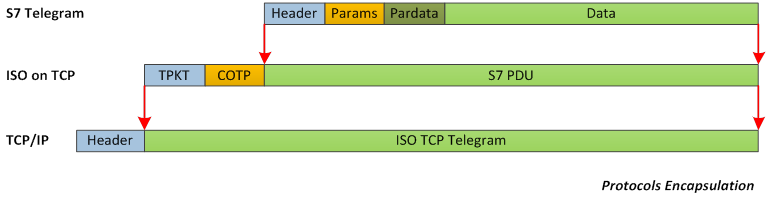
\includegraphics[width=0.85\textwidth]{img/side-sniff-image/snap7_header.png}
    \caption{Struttura multilivello di un pacchetto Siemens S7Comm (TPKT $\rightarrow$ COTP $\rightarrow$ S7).}
    \label{fig:s7_header}
  \end{figure}

  \paragraph{Handler OPC-UA}
  Il modulo \texttt{opcua\_packet\_handler} analizza il traffico TCP (porta 4840) relativo al protocollo OPC-UA.  
  Ogni pacchetto viene decodificato in base ai campi del livello applicativo: \texttt{message\_type} (HEL, ACK, OPN, MSG), \texttt{chunk\_type}, \texttt{secure\_channel\_id}, \texttt{sequence\_number}, \texttt{request\_id} e payload binario.  
  L’handler costruisce un oggetto evento contenente queste informazioni e applica un’analisi statistica sulle dimensioni e la sequenza dei pacchetti.  
  Anche qui viene utilizzato \texttt{ZScoreService} per rilevare deviazioni dai profili normali di comunicazione, segnalando eventuali anomalie al sistema centrale.  
  L’architettura è predisposta per integrare successivamente un modulo ML per la decodifica semantica del payload OPC-UA, consentendo in futuro una classificazione più profonda delle operazioni.  

  \begin{figure}[!ht]
    \centering
    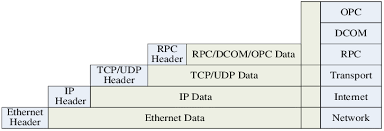
\includegraphics[width=0.85\textwidth]{img/side-sniff-image/opc_ua_header.png}
    \caption{Struttura tipica di un pacchetto OPC-UA con header applicativo e campi di sessione.}
    \label{fig:opcua_header}
  \end{figure}

  \paragraph{Sintesi operativa}
  Tutti gli handler condividono una struttura comune:
  \begin{itemize}
    \item verifica preliminare del livello di trasporto (TCP/UDP) e della porta di interesse;
    \item decodifica e parsing del payload applicativo tramite funzioni dedicate;
    \item estrazione di \textit{feature} numeriche e simboliche per il motore di analisi;
    \item analisi statistica tramite Z-Score e, se necessario, validazione con modello ML;
    \item generazione di eventi strutturati e logging di sistema.
  \end{itemize}
  Questa architettura modulare permette di aggiungere nuovi protocolli SCADA con minimo impatto sul codice principale, mantenendo la compatibilità con il Dispatcher e con il sistema di rilevamento centralizzato.


  \subsection{Decodifica dei Payload Applicativi}

Ciascun \textit{handler} di protocollo integra un modulo di \textit{decoding} dedicato per l’interpretazione dettagliata del payload applicativo, garantendo un’analisi coerente con le specifiche del protocollo industriale.  
La decodifica consente di estrarre campi semantici significativi (Function Code, Request ID, Data Block, ecc.) dai pacchetti raw e di tradurli in strutture dati interpretabili dai moduli di analisi e rilevamento anomalie.

\paragraph{Parsing Modbus/TCP}
Il decoder per il protocollo Modbus/TCP effettua la suddivisione del payload in base alla struttura MBAP e al campo funzione.  
Ogni pacchetto è composto dai seguenti elementi principali:
\begin{itemize}
  \item \textbf{Transaction ID} (2 byte): identificativo univoco della transazione;
  \item \textbf{Protocol ID} (2 byte): generalmente impostato a 0 per Modbus TCP;
  \item \textbf{Length} (2 byte): lunghezza del messaggio successivo;
  \item \textbf{Unit ID} (1 byte): indirizzo dello slave Modbus;
  \item \textbf{Function Code} (1 byte): operazione richiesta (lettura/scrittura);
  \item \textbf{Data} (variabile): contenuto del messaggio.
\end{itemize}

La funzione \texttt{parse\_modbus\_payload()} effettua l’unpacking del payload e gestisce sia le normali risposte di funzione, sia i messaggi di errore (exception codes).  
I codici funzione e le eccezioni sono mappati in dizionari interni per fornire una decodifica semantica leggibile, utile al motore di analisi statistico e ML.  
Un estratto del decoder è mostrato di seguito:

\begin{lstlisting}[language=Python, caption={Dichiarazione del channel exchange RabbitMQ in Python}, label={lst:exchange_1}]
exchange_name = "frontend.events"
channel.exchange_declare(exchange=exchange_name, exchange_type="fanout")
transaction_id, protocol_id, length = struct.unpack(">HHH", payload[:6])
unit_id = payload[6]
function_code = payload[7]
data = payload[8:]
\end{lstlisting}


\paragraph{Parsing Siemens S7 (S7Comm)}
Il decoder S7 implementa una logica multilivello conforme alla pila TPKT 
$\rightarrow$ COTP $\rightarrow$ S7Comm.  
La funzione \texttt{parse\_s7\_payload()} effettua:
\begin{enumerate}
  \item parsing dell’header TPKT (versione, lunghezza);
  \item estrazione del PDU Type e dei parametri COTP;
  \item interpretazione della PDU S7 con riferimento ai campi \texttt{ROSCTR}, \texttt{Job Function} e \texttt{Data Block}.
\end{enumerate}

Ogni pacchetto viene arricchito con metadati semantici (funzione logica, area di memoria, riferimento DB, ecc.) per consentire un’analisi ad alto livello delle operazioni PLC.  
I dizionari \texttt{S7\_JOB\_FUNCTIONS}, \texttt{S7\_MEMORY\_AREAS} e \texttt{S7\_ROSCTR} consentono di tradurre i codici numerici in descrizioni leggibili.

\paragraph{Parsing OPC-UA}
Il decoder OPC-UA gestisce la versione binaria del protocollo su TCP (porta 4840).  
La funzione \texttt{parse\_opcua\_payload()} analizza la sequenza dei campi:
\begin{itemize}
  \item \textbf{Message Type} (3 char): tipo di messaggio, come \texttt{HEL}, \texttt{ACK}, \texttt{OPN}, \texttt{MSG};
  \item \textbf{Chunk Type} (1 char): indica se il messaggio è completo o frammentato;
  \item \textbf{Secure Channel ID}, \textbf{Sequence Number}, \textbf{Request ID};
  \item \textbf{Payload}: dati applicativi codificati in formato binario.
\end{itemize}

I campi principali vengono convertiti in dizionari serializzabili per il successivo invio al motore di rilevamento.  
Questo approccio consente di effettuare un’analisi comportamentale anche sui messaggi OPC-UA, valutando pattern di frequenza, sequenza e dimensione dei pacchetti.

\paragraph{Architettura comune dei decoder}
Tutti i decoder condividono una struttura coerente:
\begin{itemize}
  \item validazione preliminare della lunghezza del payload;
  \item estrazione dei campi principali mediante \texttt{struct.unpack()};
  \item costruzione di un dizionario semantico con metadati leggibili;
  \item eventuale normalizzazione dei dati per l’analisi statistica e ML.
\end{itemize}

Questa uniformità semantica tra gli \textit{handler} permette al sistema \texttt{side-sniff} di trattare protocolli eterogenei in modo unificato, garantendo compatibilità con i moduli di rilevamento e con il sistema di alerting MQTT.

\subsection{Modulo di Anomaly Detection: Z-Score Service}
\label{subsec:zscore-service}

Il modulo \texttt{ZScoreService} rappresenta il componente statistico centrale del sistema, impiegato da ciascun \textit{Protocol Handler} per la valutazione dinamica delle anomalie nei flussi di pacchetti SCADA.  
La logica implementata si basa sull'analisi delle deviazioni standard (metrica Z-score) rispetto a valori di riferimento (\textit{baseline}) specifici per ogni coppia \texttt{device-protocol}.  

\subsubsection*{Architettura e Funzionamento}
\texttt{ZScoreService} è strutturato come una \textit{singleton class} thread-safe, garantendo l’accesso concorrente da parte di più thread di parsing provenienti dai vari \textit{handler}.  
All’avvio, il modulo inizializza un insieme di baseline statistiche di default, definendo per ciascuna metrica di interesse — come \texttt{function\_code} e \texttt{data\_length} — una media (\(\mu\)) e una deviazione standard (\(\sigma\)) di riferimento.

Ogni \textit{Protocol Handler} (es. Modbus, S7, OPC-UA) invoca il metodo \texttt{check()} passando un dizionario di \textit{features} estratte dal pacchetto corrente:
\begin{itemize}
  \item \textbf{function\_code}: operazione Modbus o tipo di servizio S7;
  \item \textbf{data\_length}: dimensione del payload;
  \item \textbf{timing features}: (opzionali) tempo di risposta o frequenza di richieste.
\end{itemize}

Per ciascuna metrica numerica, il modulo calcola il valore:
\[
Z = \frac{x - \mu}{\sigma}
\]
dove \(x\) rappresenta il valore osservato nel pacchetto corrente.  
Se il valore assoluto \(|Z|\) eccede la soglia configurata (\texttt{threshold}, di default 3), l’evento viene classificato come anomalo e accumulato in una coda temporale associata al dispositivo e protocollo di origine.

\subsubsection*{Meccanismo di Aggregazione Temporale}
Per evitare falsi positivi dovuti a fluttuazioni isolate, il modulo impiega un meccanismo di aggregazione basato su una \texttt{deque} temporale (\textit{sliding window}) di dimensione configurabile (\texttt{aggregation\_window}).  
Solo quando il numero minimo di anomalie (\texttt{min\_anomalies}) viene superato all’interno della finestra temporale, viene generato un evento di allarme consolidato, notificato al sistema superiore di alerting.

\subsubsection*{Aggiornamento Dinamico delle Baseline}
Il modulo supporta un aggiornamento adattivo delle baseline, attivabile tramite il flag \texttt{update\_dynamic=True}.  
In tale modalità, le statistiche vengono aggiornate in tempo reale secondo due strategie:
\begin{enumerate}
  \item \textbf{Media Mobile Esponenziale (EMA)}: attivata con il parametro \texttt{use\_ema=True}, utilizza un coefficiente \(\alpha\) per dare maggiore peso agli eventi recenti:
  \[
  \mu_{t} = \alpha x_{t} + (1 - \alpha) \mu_{t-1}
  \]
  \item \textbf{Aggiornamento Lineare Medio}: in alternativa, viene calcolata una media aritmetica progressiva dei valori recenti per una stabilizzazione graduale.
\end{enumerate}

\subsubsection*{Gestione della Concorrenza e Persistenza}
L’intero accesso ai dati condivisi (statistiche, soglie, anomalie) è protetto da un \texttt{Lock} per garantire la coerenza in ambienti multithread, specialmente quando più \textit{handler} aggiornano simultaneamente le stesse strutture dati.  
Le baseline e le soglie possono inoltre essere personalizzate per singolo dispositivo o protocollo attraverso i metodi:
\begin{itemize}
  \item \texttt{set\_baseline(device\_id, protocol, baseline\_stats)}
  \item \texttt{set\_threshold(device\_id, protocol, threshold)}
\end{itemize}

\subsubsection*{Integrazione con i Protocol Handler}
Ciascun \textit{handler} invoca \texttt{ZScoreService.get\_instance().check()} durante la fase di analisi di ogni pacchetto decodificato.  
Se la funzione restituisce un’anomalia aggregata, il messaggio generato viene inviato al modulo di \textit{alert management}, che può inoltrarlo via MQTT o loggarlo nel sistema SIEM.  
Questo approccio permette un’analisi statistica coerente e centralizzata, indipendentemente dal tipo di protocollo in uso.

\subsubsection*{Sintesi Operativa}
Il flusso di funzionamento può essere riassunto come segue:
\begin{enumerate}
  \item L’handler decodifica il pacchetto e ne estrae le feature numeriche;
  \item Le feature vengono inviate al modulo \texttt{ZScoreService};
  \item Viene calcolato lo Z-score per ogni metrica;
  \item Le anomalie vengono accumulate e analizzate in una finestra temporale;
  \item Al superamento della soglia di aggregazione viene generato un evento di allarme.
\end{enumerate}


\end{enumerate}


\subsection{Flusso di Comunicazione: side-sniff e side-device-discovery}

Il modulo \texttt{side-sniff} è responsabile della cattura dei pacchetti in tempo reale all’interno dell’ambiente ICS/SCADA.  
Una volta decodificati, i pacchetti vengono pubblicati in un canale di messaggistica intermedio, consumato dal servizio \texttt{side-device-discovery}.  

Quest’ultimo agisce da \textit{intermediario logico} tra il livello di cattura e il backend, svolgendo le seguenti funzioni:
\begin{itemize}
    \item \textbf{Consumer}: riceve i messaggi dal \texttt{side-sniff}, contenenti informazioni grezze o pre-elaborate.
    \item \textbf{Publisher}: invia al modulo \texttt{side-api-back-end} eventi arricchiti con metadati e risultati statistici provenienti dallo \texttt{ZScoreService} o dai vari modelli di machine learning individuali.
\end{itemize}

\begin{figure}[!ht]
    \centering
    \begin{tikzpicture}[
        node distance=4cm and 1.5cm,
        every node/.style={font=\sffamily, align=center},
        box/.style={
            draw, 
            thick, 
            rounded corners, 
            text centered, 
            minimum height=1.2cm, 
            minimum width=3.5cm, 
            fill=blue!5
        },
        arrowmqtt/.style={
            -{Stealth[length=3mm, width=2mm]},
            ultra thick,
            red
        },
        arrowdb/.style={
            -{Stealth[length=3mm, width=2mm]},
            ultra thick,
            orange
        },
        scale=0.75, transform shape
    ]

    % --- Nodi principali ---
    \node[box, fill=green!20] (sniff) {\texttt{side-sniff}};
    \node[box, fill=yellow!20, right=of sniff] (discovery) {\texttt{side-device-discovery}};
    \node[box, fill=red!20, right=of discovery] (backend) {\texttt{side-api-back-end}};
    \node[box, fill=orange!20, below=of discovery] (db) {
\includegraphics[width=2.5cm]{img/side-sniff-image/neo4_logo.png}\\Neo4j Database};

    % --- Frecce principali ---
    \draw[arrowmqtt] (sniff) -- (discovery);
    \draw[arrowmqtt] (discovery) -- (backend);
    \draw[arrowdb] (discovery) -- (db);

    \end{tikzpicture}

    \vspace{0.3cm}
    \small
    \begin{tabular}{rl}
        \textcolor{red}{\rule[0.5ex]{1cm}{1pt}} & Comunicazione tramite \textbf{MQTT} \\
        \textcolor{orange}{\rule[0.5ex]{1cm}{1pt}} & Interazione con il \textbf{Database Neo4j}
    \end{tabular}

    \caption{Flusso di comunicazione semplificato tra i moduli principali e il database.}
    \label{fig:side-sniff-discovery-backend-db}
\end{figure}


%%%%%%%%%%%%%%%%%%%%%%%%%%%%%%%%%%%%%%



%%% Side-Device-Discovery
\section{side-device-discovery}

Il modulo \texttt{side-device-discovery} è progettato come servizio in background, il cui scopo principale è quello di ricevere e gestire gli eventi pubblicati dal modulo \texttt{side-sniff}, consentendo successivamente la loro distribuzione verso i moduli di backend e front-end. In questo modo, \texttt{side-device-discovery} funge sia da \textbf{consumer} che da \textbf{publisher} nel flusso di comunicazione del sistema.

\subsection{Funzionamento generale}

Il modulo si comporta come un servizio persistente che esegue le seguenti operazioni:
\begin{enumerate}
    \item Si collega a un broker RabbitMQ per consumare gli eventi pubblicati dal modulo \texttt{side-sniff}.
    \item Processa ciascun evento tramite handler registrati dinamicamente, distinguendo i tipi di evento (ad esempio, \texttt{new\_device} o \texttt{device\_update}).
    \item Inserisce o aggiorna le informazioni sui dispositivi all'interno del database Neo4j, mantenendo la topologia dei dispositivi e le relazioni di comunicazione.
    \item Pubblica gli eventi elaborati su un exchange dedicato verso i moduli \texttt{side-api-back-end} e \texttt{side-front-end}.
\end{enumerate}

\subsection{Struttura del codice}

Il modulo è composto principalmente dai seguenti file e componenti:

\paragraph{1. \texttt{side-device-discovery.py}}  
Questo script rappresenta il cuore del modulo. Le sue funzioni principali sono:
\begin{itemize}
    \item \textbf{Registrazione degli handler:} tramite il decorator \texttt{register\_handler} ogni funzione viene associata a una \texttt{routing\_key}, consentendo la gestione dinamica degli eventi ricevuti.
    \item \textbf{Callback dei messaggi:} ogni messaggio ricevuto da RabbitMQ viene elaborato tramite la funzione \texttt{callback}, che richiama l'handler corrispondente e passa il driver Neo4j per la persistenza.
    \item \textbf{Inizializzazione del servizio:} il modulo si collega a RabbitMQ, dichiara l'exchange \texttt{discovery.events} e crea una coda temporanea per ricevere tutti i messaggi dei routing key registrati.
    \item \textbf{Gestione terminazione:} viene gestita la chiusura sicura di connessioni al broker e al database in caso di interruzione.
\end{itemize}

\paragraph{2. \texttt{services/database\_service.py}}  
Contiene la funzione \texttt{register\_modbus\_event} che gestisce l'upsert dei nodi e delle relazioni all'interno del database Neo4j. In particolare:
\begin{itemize}
    \item Crea o aggiorna i nodi dei dispositivi (\texttt{NODE\_DEVICE}) identificati da IP e porta.
    \item Definisce le relazioni bidirezionali (\texttt{RELATION\_COMMUNICATES\_WITH}) tra dispositivi, memorizzando informazioni come protocollo, timestamp e conteggio degli eventi.
    \item Supporta la persistenza di dati Modbus, ma può essere esteso ad altri protocolli.
\end{itemize}

\paragraph{3. \texttt{configuration/device\_discovery\_publisher.py}}  
Implementa il servizio di pubblicazione verso RabbitMQ:
\begin{itemize}
    \item Inizializza una connessione al broker e dichiara un \texttt{exchange} di tipo \texttt{fanout}.
    \item Permette la pubblicazione di eventi elaborati verso tutti i subscriber collegati.
    \item Gestisce la chiusura sicura della connessione.
\end{itemize}

\subsection{Flusso operativo}

Il flusso operativo del modulo può essere sintetizzato come segue:

\begin{enumerate}
    \item \texttt{side-sniff} pubblica un messaggio contenente le informazioni dei pacchetti catturati.
    \item \texttt{side-device-discovery} riceve il messaggio tramite RabbitMQ e lo passa al handler registrato.
    \item L'handler utilizza il driver Neo4j per aggiornare la rappresentazione dei dispositivi e delle loro relazioni.
    \item Il messaggio elaborato viene pubblicato sull'exchange \texttt{frontend.events}, rendendolo disponibile per i moduli di backend e frontend.
\end{enumerate}

\subsection{Proprietà principali}

\begin{itemize}
    \item Funziona come servizio in background persistente.
    \item Gestisce eventi di tipo \texttt{new\_device} e \texttt{device\_update}.
    \item Interagisce direttamente con il database Neo4j per garantire la consistenza dei dati dei dispositivi.
    \item Pubblica eventi verso sistemi downstream tramite RabbitMQ, implementando un pattern \textit{publish-subscribe}.
\end{itemize}


%%% Side - API - Back-End
\section{side-api-backend}

Il modulo \texttt{side-api-back-end} costituisce il componente di interfaccia tra il \textit{core system} e il \textit{front-end} dell’ambiente S.I.D.E. (SCADA Intrusion Detection Environment).  
È implementato come server \texttt{FastAPI} eseguibile tramite \texttt{Uvicorn}, e integra in un unico livello applicativo:
\begin{enumerate}
  \item la gestione delle connessioni WebSocket per la comunicazione in tempo reale con l’interfaccia utente;
  \item l’esposizione di API REST per interrogazioni dirette (es. elenco dispositivi, relazioni, metriche);
  \item la gestione della persistenza e della topologia di rete su database \texttt{Neo4j};
  \item l’integrazione asincrona con il broker \texttt{RabbitMQ} per la ricezione di eventi generati dai moduli di scoperta e analisi.
\end{enumerate}

\subsection{Struttura generale}
La struttura principale del modulo è organizzata nei seguenti componenti:
\begin{itemize}
  \item \textbf{run.py}: punto d’ingresso del server applicativo;
  \item \textbf{configuration/}: contiene le impostazioni di sistema e i moduli di inizializzazione (database, WebSocket);
  \item \textbf{services/}: implementa la logica di business (query Neo4j, formattazione dati);
  \item \textbf{controllers/}: definisce gli endpoint REST e WebSocket esposti al front-end;
  \item \textbf{service\_discovery\_consumer.py}: gestisce un processo di ascolto RabbitMQ per l’inoltro di eventi in tempo reale al front-end.
  \item \textbf{service\_discovery\_alert\_consumer.py}: gestisce un processo di ascolto RabbitMQ per l'inoltro di eventi di alert in tempo reale al front-end. 
  \item \textbf{websocket\_manager.py}: gestisce due weboscket per l'inoltro dei messaggi arrivati dai canali di comunicazione di RabbitMQ 
\end{itemize}

\subsection{Punto di avvio: \texttt{run.py}}
Il file \texttt{run.py} costituisce il \textit{bootstrap} del server.  
Esso costruisce dinamicamente il riferimento all’applicazione \texttt{FastAPI} utilizzando i parametri definiti nel file di configurazione:

\begin{lstlisting}[language=Python, caption={Setting up iniziale del server fastapi}]

  app_location = f"{MODULE_NAME}:{APP_NAME}"


  uvicorn.run(app_location, host=HOST, port=PORT, reload=RELOAD)

\end{lstlisting}

Il server è lanciato tramite \texttt{Uvicorn}, un web server asincrono compatibile con ASGI (\textit{Asynchronous Server Gateway Interface}), che consente una gestione concorrente efficiente delle richieste.

\subsection{Gestione del database Neo4j}
Il modulo \texttt{configuration/database\_configuration.py} implementa la connessione al database a grafo \texttt{Neo4j} mediante il driver ufficiale \texttt{neo4j-driver}.  
L’inizializzazione del driver è effettuata tramite la funzione:

\begin{lstlisting}[language=Python, caption={Dichiarazione dei driver NEO4J in Python}, label={lst:exchange}]
driver = GraphDatabase.driver(URI, auth=(USER, PASSWORD))
\end{lstlisting}

I parametri di connessione vengono caricati da file \texttt{.env} per garantire la separazione tra codice e configurazione.  
La classe \texttt{SideDatabaseConfiguration} incapsula i parametri di connessione e offre metodi getter/setter validati.  
Il modulo definisce inoltre le entità principali (\texttt{Device}) e le relazioni (\texttt{COMMUNICATES\_WITH}) utilizzate per modellare le topologie ICS/SCADA, includendo proprietà quali:
\begin{itemize}
  \item \texttt{ip}, \texttt{port}, \texttt{role}, \texttt{protocol}, \texttt{first\_seen}, \texttt{last\_seen} per i nodi \texttt{Device};
  \item \texttt{protocol}, \texttt{total\_queries}, \texttt{error\_count} e \texttt{queries\_by\_function} per le relazioni di comunicazione.
\end{itemize}

\subsection{Gestione degli eventi asincroni: \texttt{service\_discovery\_consumer.py}}
Il file \texttt{service\_discovery\_consumer.py} avvia un \texttt{RabbitMQ consumer} per ricevere notifiche e aggiornamenti di rete provenienti dal modulo \texttt{ServiceDiscovery} o da altri microservizi.  
Utilizza la libreria \texttt{pika} per instaurare una connessione al broker, sottoscrivendosi all’exchange:
\begin{lstlisting}[language=Python, caption={Dichiarazione dell'exchange RabbitMQ in Python}, label={lst:exchange}]
exchange_name = "frontend.events"
channel.exchange_declare(exchange=exchange_name, exchange_type="fanout")
\end{lstlisting}
Ogni messaggio ricevuto viene deserializzato (formato JSON) e inoltrato in modo asincrono al gestore WebSocket \texttt{ws\_manager.broadcast(event)}, garantendo un flusso in tempo reale verso i client front-end connessi.

\subsection{Gestione connessioni WebSocket: \texttt{websocket\_manager.py}}
Il componente \texttt{WebSocketManager} fornisce una gestione centralizzata delle connessioni WebSocket attive.  
È responsabile della ricezione e dell’invio dei messaggi tra il back-end e i client:
\begin{itemize}
  \item \texttt{connect(ws)}: accetta una nuova connessione;
  \item \texttt{disconnect(ws)}: rimuove connessioni interrotte;
  \item \texttt{broadcast(message)}: invia in broadcast messaggi JSON a tutti i client attivi.
\end{itemize}
Il manager mantiene le connessioni attive in un set tipizzato \texttt{Set[WebSocket]}, assicurando la scalabilità anche in presenza di più sessioni contemporanee.

\subsection{Controller REST e WebSocket}
Due controller principali orchestrano la comunicazione:
\begin{enumerate}
  \item \textbf{\texttt{graph\_controller.py}} — espone endpoint REST come \texttt{/api/devices}, che interroga Neo4j tramite il servizio \texttt{get\_devices(driver)} e restituisce la topologia o i dispositivi attivi;
  \item \textbf{\texttt{websocket\_controller.py}} — gestisce il canale \texttt{/ws/network}, accettando connessioni bidirezionali e mantenendole attive per lo streaming continuo di dati (eventi, metriche, anomalie).
\end{enumerate}

\subsection{Integrazione dei servizi e funzionamento complessivo}
Il modulo \texttt{side-api-back-end} funge da \textit{orchestratore asincrono}, integrando servizi eterogenei:
\begin{itemize}
  \item riceve in tempo reale eventi e notifiche di scoperta rete via \texttt{RabbitMQ};
  \item li inoltra istantaneamente ai client tramite \texttt{WebSocketManager};
  \item fornisce API REST per consultare lo stato della rete, dispositivi e metriche analitiche;
  \item interagisce con il database \texttt{Neo4j} per aggiornare nodi e relazioni in base agli eventi ricevuti.
\end{itemize}
Questo consente al front-end di ottenere una rappresentazione dinamica della rete ICS monitorata, in cui dispositivi, connessioni e allarmi vengono aggiornati in tempo reale senza necessità di polling continuo.

\subsection{Sintesi del flusso operativo}
\begin{enumerate}
  \item Il modulo viene avviato tramite \texttt{python run.py};
  \item \texttt{Uvicorn} avvia l’applicazione \texttt{FastAPI};
  \item Il consumer RabbitMQ ascolta sull’exchange \texttt{frontend.events};
  \item Gli eventi ricevuti vengono trasmessi ai client via WebSocket;
  \item Le API REST permettono al front-end di interrogare lo stato della rete e le entità Neo4j.
\end{enumerate}

\subsection{Ruolo architetturale}
Il modulo \texttt{side-api-backend} rappresenta il \textit{nodo di interfaccia logico} tra il sistema di rilevamento (livello back-end) e il sistema di visualizzazione (front-end).  
Funge da punto unico di ingresso per tutti i dati, trasformando eventi di basso livello (pacchetti, relazioni, metriche) in strutture semantiche comprensibili al front-end, mantenendo un modello coerente della rete e dei flussi di comunicazione industriali.


\subsection{Flusso di Interazione con il Backend}

Il modulo \texttt{side-api-back-end} riceve gli eventi già filtrati ed elaborati.  
A questo livello vengono aggregati i risultati provenienti dai vari protocolli e memorizzati nel database centrale.  
Ogni evento include le informazioni statistiche fornite dal \texttt{ZScoreService}, integrato direttamente nel modulo \texttt{side-sniff}, consentendo una visione globale dello stato dei dispositivi.

\begin{figure}[!h]
    \centering
    \begin{tikzpicture}[
        node distance=4.5cm and 2cm,
        every node/.style={font=\sffamily, align=center},
        box/.style={
            draw, 
            thick, 
            rounded corners, 
            text centered, 
            minimum height=1.2cm, 
            minimum width=3.8cm, 
            fill=blue!5
        },
        arrowmqtt/.style={
            -{Stealth[length=3mm, width=2mm]},
            ultra thick,
            red
        },
        arrowws/.style={
            -{Stealth[length=3mm, width=2mm]},
            ultra thick,
            green!70!black
        },
        arrowdb/.style={
            <->, ultra thick, orange
        },
        scale=0.8, transform shape
    ]

    % --- Nodi principali ---
    \node[box, fill=green!20] (sniff) {\texttt{side-sniff}};
    \node[box, fill=yellow!20, right=of sniff] (discovery) {\texttt{side-device-discovery}};
    \node[box, fill=red!20, right=of discovery] (backend) {\texttt{side-api-back-end}};
    \node[box, fill=cyan!20, below=of backend] (frontend) {\texttt{side-front-end}};
    \node[box, fill=orange!20, below=of discovery, yshift=-2.5cm] (db) {
\includegraphics[width=2.5cm]{img/side-sniff-image/neo4_logo.png}\\Neo4j Database};

    % --- Frecce principali ---
    \draw[arrowmqtt] (sniff) -- (discovery);
    \draw[arrowmqtt] (discovery) -- (backend);
    \draw[arrowws] (backend) -- (frontend);
    \draw[arrowdb] (backend) -- (db);

    \end{tikzpicture}

    \vspace{0.3cm}
    \small
    \begin{tabular}{rl}
        \textcolor{red}{\rule[0.5ex]{1cm}{1pt}} & Comunicazione tramite \textbf{MQTT} \\
        \textcolor{green!70!black}{\rule[0.5ex]{1cm}{1pt}} & Comunicazione tramite \textbf{WebSocket} (verso il front-end) \\
        \textcolor{orange}{\rule[0.5ex]{1cm}{1pt}} & Interazione bidirezionale con il \textbf{Database Neo4j}
    \end{tabular}

    \caption{Flusso semplificato tra i moduli principali del sistema, con interazione bidirezionale tra \texttt{side-device-discovery} e il database Neo4j.}
    \label{fig:side-architecture-db-flow}
\end{figure}






\section{side-frontend}

Il modulo \textit{frontend} è sviluppato in \textbf{Next.js} e rappresenta l’interfaccia grafica principale del sistema \textbf{S.I.D.E. (SCADA Intrusion Detection Environment)}.
Il suo obiettivo è fornire una visualizzazione interattiva e in tempo reale della rete SCADA, consentendo all’operatore di monitorare in modo immediato lo stato dei dispositivi, le comunicazioni attive e gli eventi di sicurezza rilevati.

\subsection{Dashboard interattiva}
Appena effettuato l’accesso, l’operatore viene accolto da una \textbf{dashboard dinamica} che mostra la topologia della rete SCADA.
Attraverso una connessione \texttt{WebSocket} con il modulo \textit{side-api-backend}, il frontend riceve continuamente aggiornamenti riguardanti lo stato dei dispositivi e li rappresenta graficamente in un \textbf{grafo 3D interattivo}.
In questa vista è possibile osservare in tempo reale le interazioni tra \textit{client/server} (o \textit{master/slave}), con i nodi che rappresentano i dispositivi e gli archi che indicano le comunicazioni attive.
Eventuali anomalie o stati di allerta vengono evidenziati tramite codici colore o icone distintive, facilitando un’immediata comprensione della situazione di rete.

\begin{figure}[!ht]
\centering
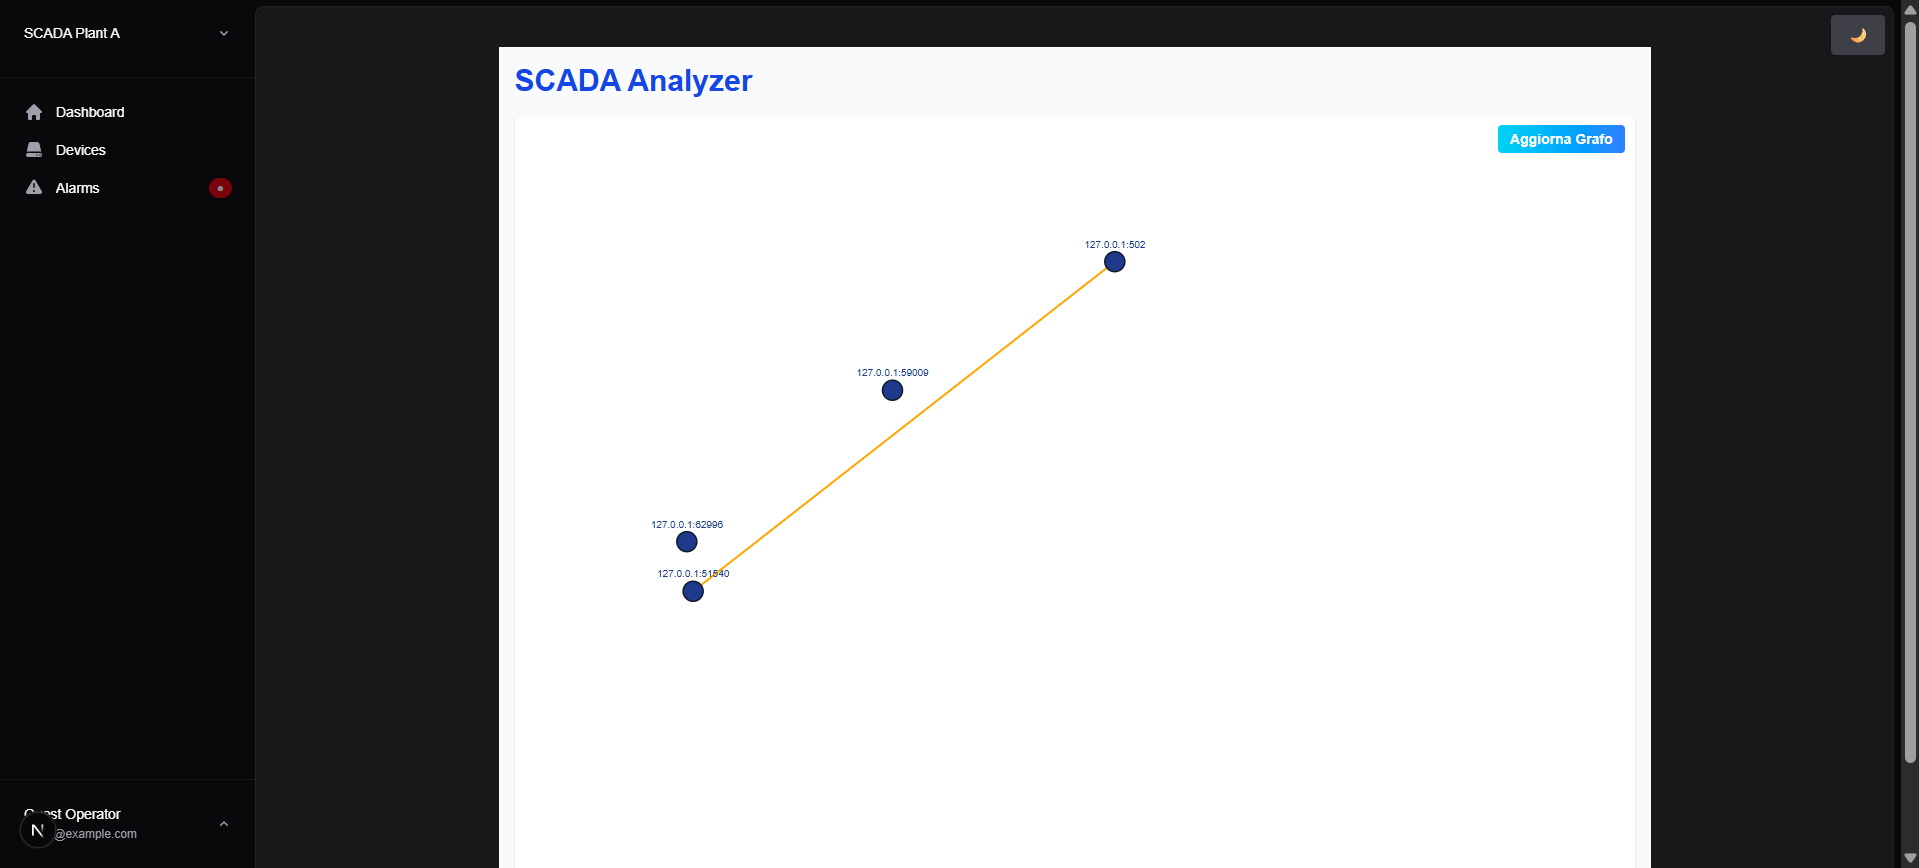
\includegraphics[width=0.8\textwidth]{img/side-frontend/dashboard_example.png}
\caption{Dashboard 3D interattiva della rete SCADA: i nodi rappresentano i dispositivi, mentre gli archi mostrano le comunicazioni attive.}
\label{fig:frontend_dashboard}
\end{figure}

\subsection{Sezione \texttt{/devices}}
All’interno della sezione \textit{/devices}, l’utente può consultare l’elenco completo dei dispositivi monitorati.
I device vengono automaticamente categorizzati in base al protocollo industriale rilevato (\texttt{Modbus}, \texttt{OPC-UA}, \texttt{S7}) e possono essere filtrati dinamicamente.
Ogni dispositivo è rappresentato tramite una \textbf{card informativa} che mostra:
\begin{itemize}
\item indirizzo IP e porta di comunicazione;
\item ruolo nel sistema (client/server);
\item stato corrente (\textit{attivo} o \textit{inattivo});
\item protocollo di riferimento.
\end{itemize}

\begin{figure}[!ht]
\centering
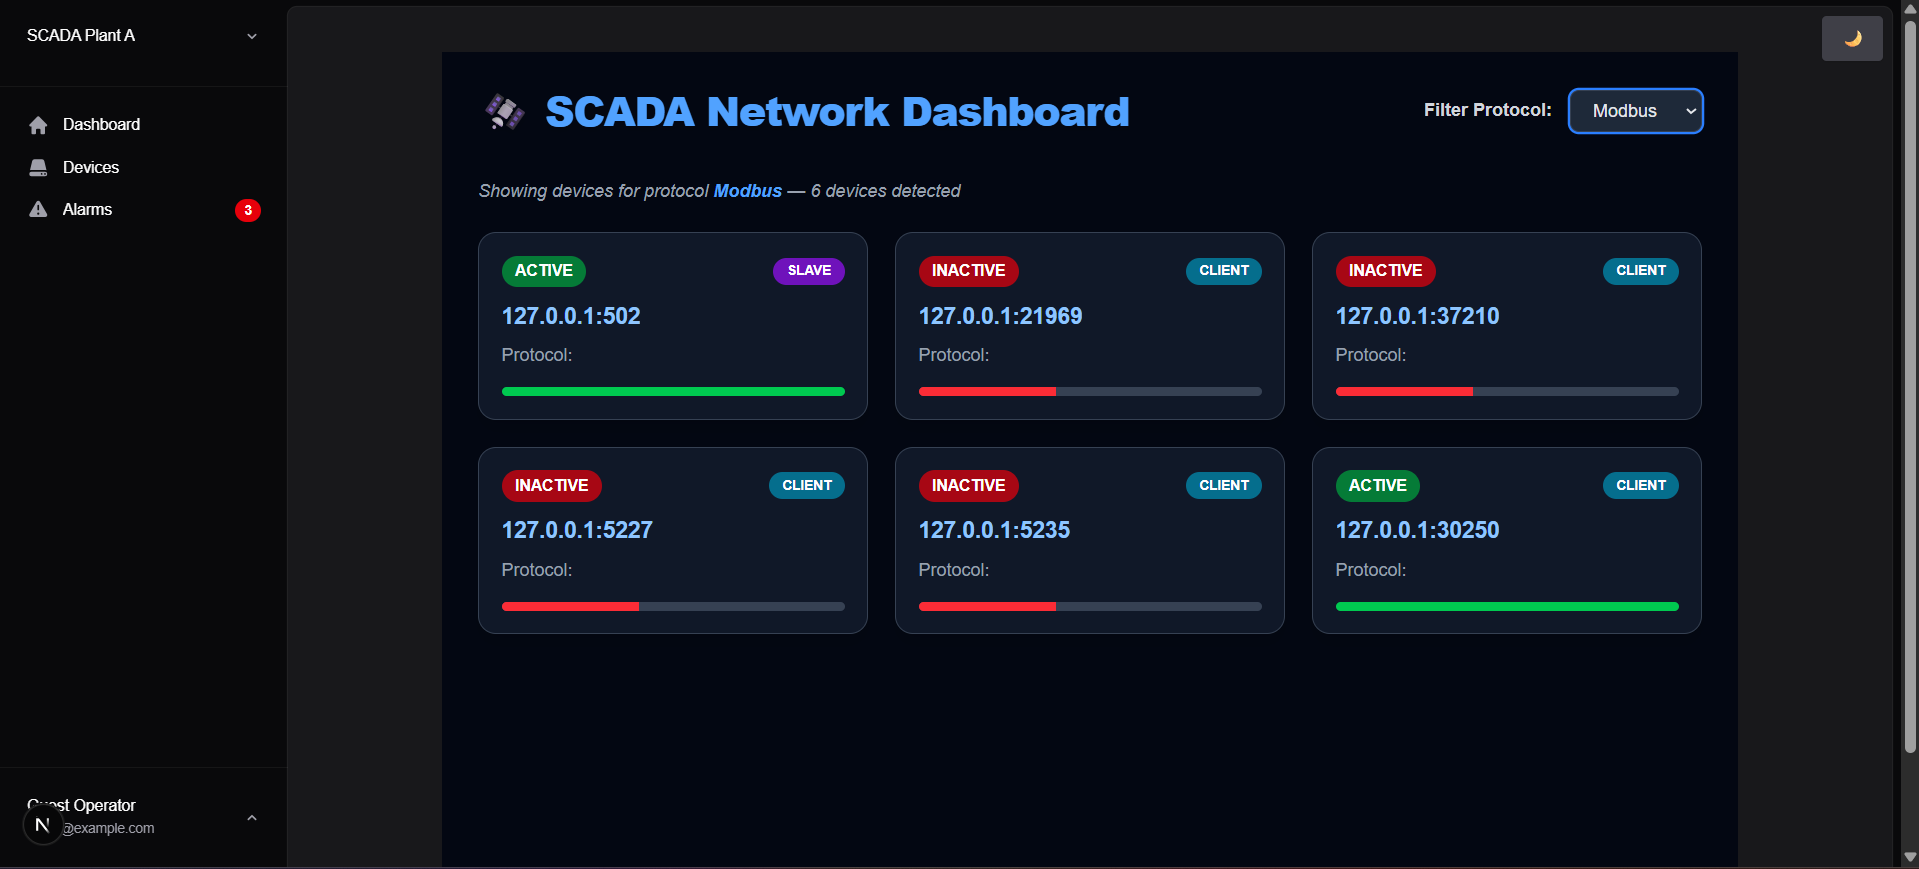
\includegraphics[width=0.8\textwidth]{img/side-frontend/devices_example.png}
\caption{Visualizzazione dei dispositivi SCADA e relativo filtraggio per protocollo.}
\label{fig:frontend_devices}
\end{figure}

\subsection{Sezione \texttt{/events}}
La sezione dedicata agli \textit{eventi} o \textit{allarmi} consente di analizzare in dettaglio le segnalazioni di sicurezza.
Tramite un sistema di filtraggio basato sulla \textbf{severity} dell’evento (ad esempio \texttt{EARLY\_WARNING\_ZSCORE} o \texttt{CONFIRMED\_ANOMALY\_ML}), l’operatore può isolare rapidamente gli episodi di interesse.
Ogni evento può essere espanso in una card dedicata che mostra:
\begin{itemize}
\item il tipo di anomalia rilevata;
\item il dispositivo coinvolto e il protocollo di riferimento;
\item la descrizione dettagliata del pacchetto o dei dati analizzati.
\end{itemize}

\begin{figure}[!ht]
    \centering
    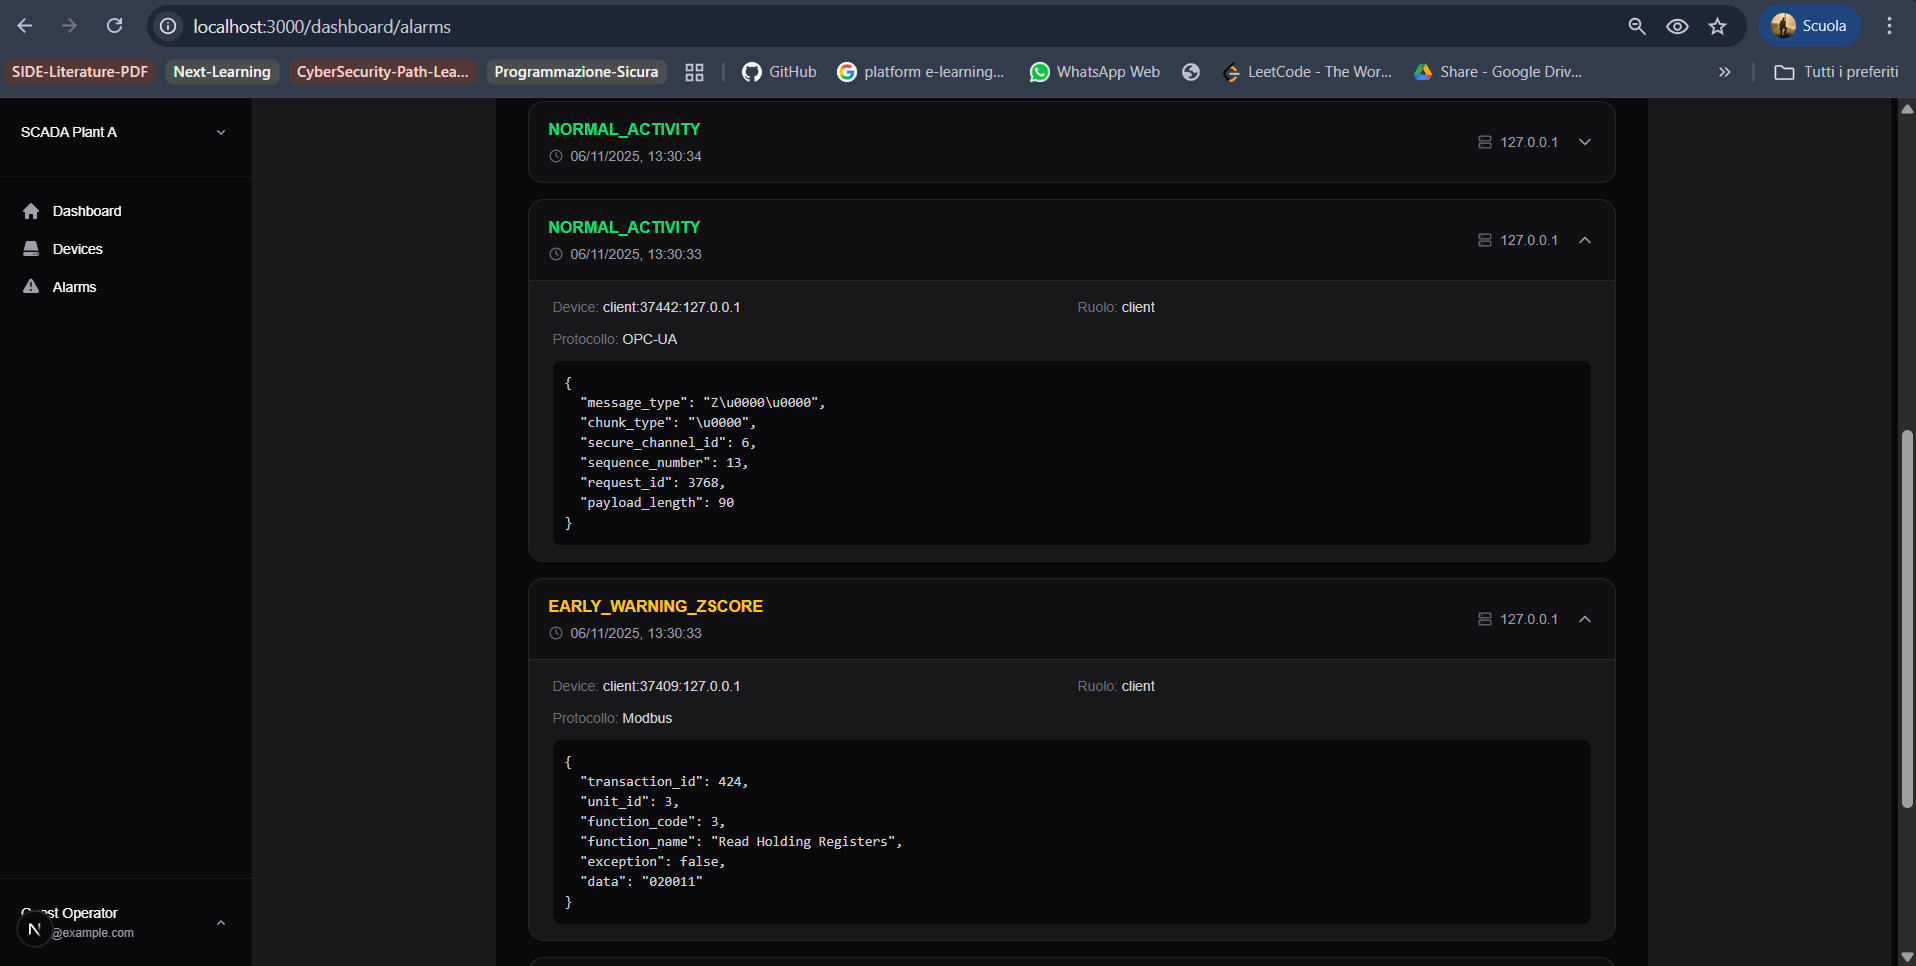
\includegraphics[width=0.8\textwidth]{img/side-frontend/devices_alarms_zscore.png}
    \caption{Visualizzazione dei vari eventi attraverso livelli di Severity}
    \label{fig:neo4j_dashboard}
\end{figure}



Questo consente una comprensione approfondita del contesto operativo e del comportamento anomalo individuato dal sistema di rilevazione.

Un altro componente grafico molto intuitivo è quello di \textbf{Neo4J}, che supporta la visualizzazione dei dati memorizzati nel database a grafo.  
Nel grafo sono rappresentati i seguenti nodi principali:
\begin{itemize}
    \item \textbf{Device} — rappresenta un dispositivo presente nella rete SCADA;
    \item \textbf{Anomaly} — indica un evento anomalo rilevato dai moduli di analisi (Z-Score o Machine Learning).
\end{itemize}

Le relazioni tra i nodi sono invece:
\begin{itemize}
    \item \texttt{COMMUNICATES\_WITH} — indica le comunicazioni attive tra due dispositivi;
    \item \texttt{HAS\_EVENTS} — collega un dispositivo agli eventi o alle anomalie rilevate durante l’interazione.
\end{itemize}

\begin{figure}[!ht]
    \centering
    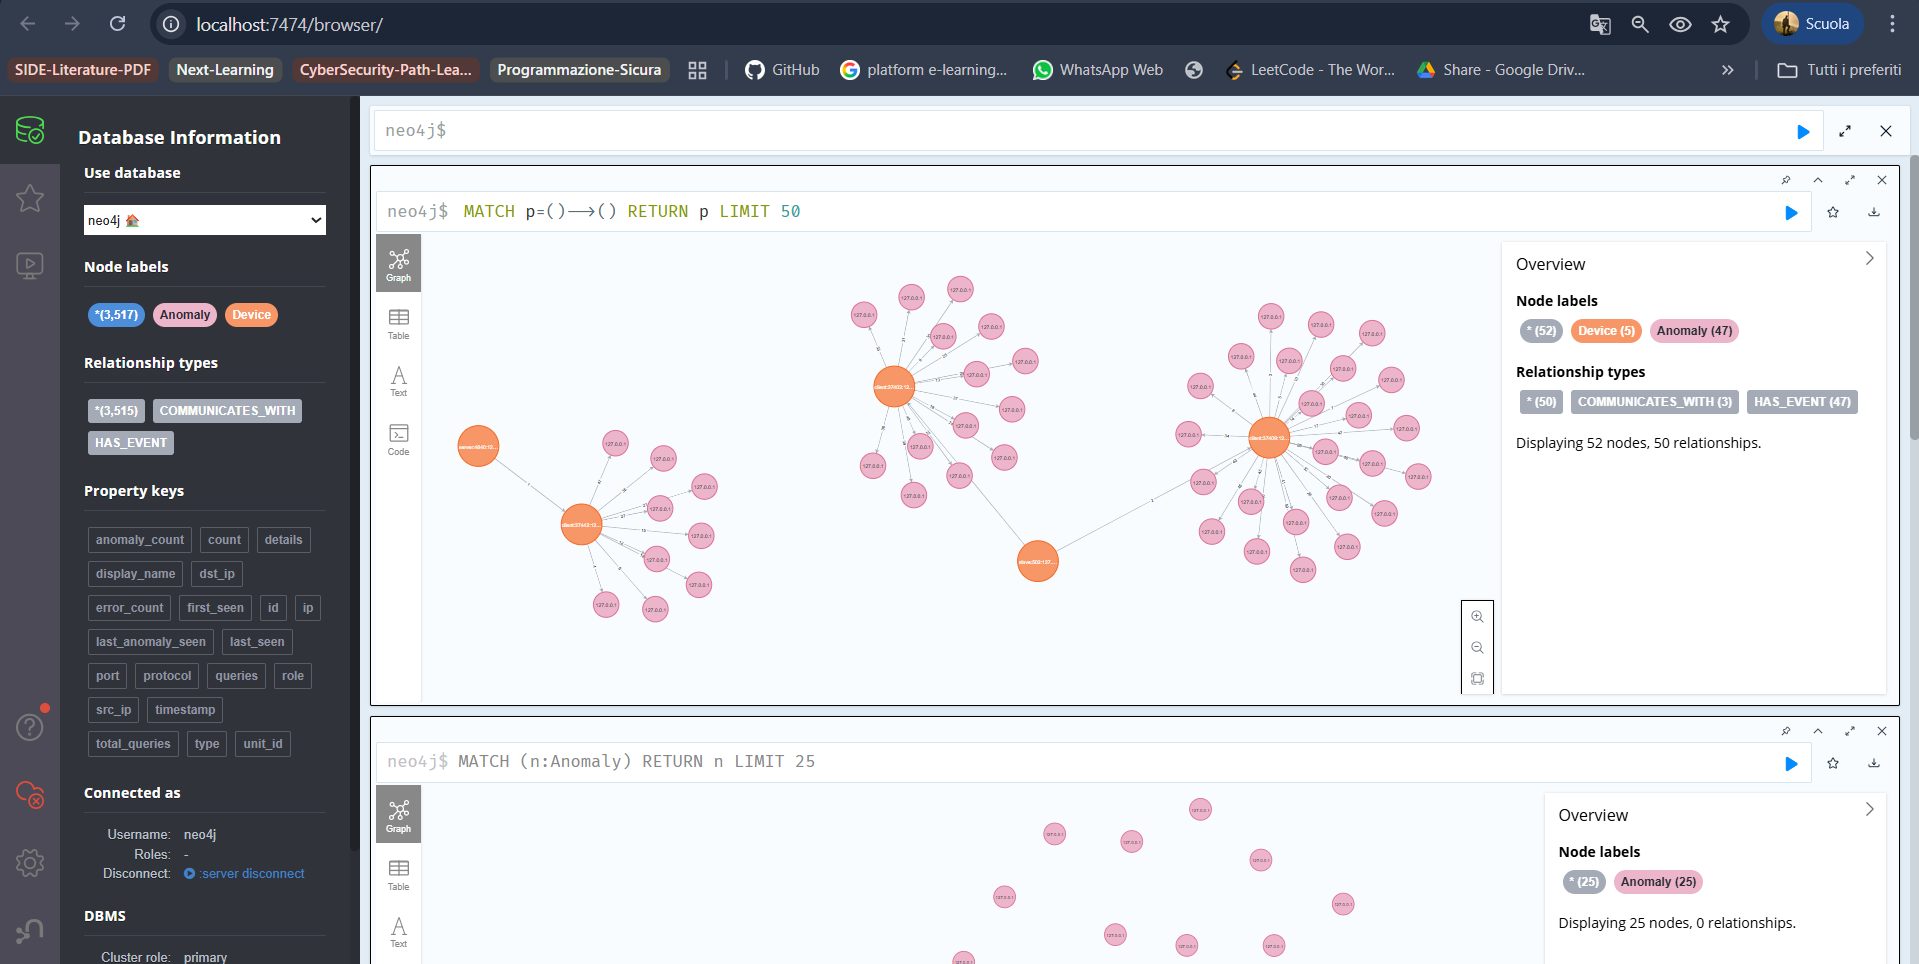
\includegraphics[width=0.8\textwidth]{img/side-frontend/dashboard_neo4j.png}
    \caption{Visualizzazione del grafo dei dispositivi e delle anomalie in Neo4J.}
    \label{fig:neo4j_dashboard}
\end{figure}

Questa rappresentazione consente di comprendere rapidamente la frequenza e la distribuzione degli eventi nella rete, distinguendo tra anomalie leggere (rilevate tramite \textit{Z-Score}) e anomalie gravi (individuate tramite modelli di \textit{Machine Learning}, come l’\textit{Isolation Forest}).



\subsection{Avvio del modulo}
Per avviare il modulo \textit{frontend}, è sufficiente installare la versione LTS \texttt{v22.16.0} di Node.js, accedere alla directory del progetto ed eseguire il comando:
\begin{verbatim}
npm run dev
\end{verbatim}





\section{side-ml-models}
\label{ch:side_ml_models}

All'interno del modulo \texttt{side-ml-models}, il processo di addestramento del modello di rilevazione anomalie si articola in due fasi principali: estrazione dei dati dai file \texttt{PCAP} e training del modello \texttt{Isolation Forest}.

\subsection{Estrazione dei dati dai file PCAP}

I pacchetti di rete catturati in contesti SCADA/ICS sono organizzati nella cartella \texttt{data-modbus}. L'elaborazione dei pacchetti avviene mediante lo script \texttt{pcap\_to\_csv\_enhanced.py}, che realizza le seguenti operazioni:

\begin{enumerate}
    \item \textbf{Scansione dei file PCAP:} tutti i file nella directory \texttt{data-modbus} vengono letti e processati in sequenza.
    \item \textbf{Parsing dei protocolli:} identificazione di ARP, IP, TCP, UDP e ICMP, con estrazione delle principali feature:
    \begin{itemize}
        \item \texttt{src\_ip}, \texttt{dst\_ip}
        \item \texttt{src\_port}, \texttt{dst\_port}
        \item \texttt{pkt\_size}, \texttt{ip\_ttl}, \texttt{ip\_proto\_num}
    \end{itemize}
    \item \textbf{Parsing Modbus TCP:} per i pacchetti con porta TCP 502, estrazione di:
    \begin{itemize}
        \item \texttt{function\_code}, \texttt{data\_length}
        \item eventuali eccezioni (\texttt{exception\_code}, \texttt{exception\_message})
    \end{itemize}
    \item \textbf{Creazione del dataset:} i dati estratti vengono convertiti in CSV tramite un DataFrame Pandas, includendo un file di riepilogo con statistiche sulle feature principali.
\end{enumerate}

\subsection{Addestramento del modello Isolation Forest}

Il dataset CSV ottenuto viene utilizzato per addestrare un modello \texttt{Isolation Forest}, con le seguenti fasi:

\begin{enumerate}
    \item \textbf{Selezione dei dati di training:} dal dataset di attacco, il 70\% dei record viene scelto per l'addestramento; il restante 30\% può essere utilizzato per validazione.
    \item \textbf{Preprocessing:} le feature numeriche vengono standardizzate mediante \texttt{StandardScaler} fit solo sui dati d'attacco.
    \item \textbf{Addestramento:} il modello Isolation Forest viene addestrato sui dati standardizzati, con parametri configurabili (\texttt{n\_estimators}, \texttt{contamination}).
    \item \textbf{Determinazione della soglia:} la soglia di decisione viene calcolata come percentile specifico dei punteggi di training (\texttt{decision\_function}), utile per valutare anomalie tramite Z-Score.
    \item \textbf{Valutazione:} test del modello sul sottoinsieme di attacchi residui e sul dataset clean, calcolando la percentuale di falsi positivi e visualizzando la distribuzione dei punteggi.
    \item \textbf{Salvataggio degli artefatti:} modello, scaler e soglia vengono serializzati e salvati su disco in formato \texttt{.joblib}, permettendo l’integrazione all’interno dei diversi Handler di rilevazione anomalie.
\end{enumerate}

\subsection{Osservazioni}

Ogni Handler dispone di un modello singolo e univoco, addestrato su dataset differenti selezionati in base alla tipologia di protocollo (ad esempio \texttt{Modbus}, \texttt{OPC-UA}, \texttt{S7}).  
Grazie alla serializzazione in \texttt{.joblib}, ogni Handler può caricare il proprio modello in fase di esecuzione e valutare in tempo reale se un evento supera la soglia di Z-Score, permettendo l’attivazione di allarmi o trigger specifici.  

Questa struttura garantisce:

\begin{itemize}
    \item la modularità dei modelli per protocollo, evitando conflitti tra diverse tipologie di traffico;
    \item la possibilità di aggiornare o riaddestrare singoli modelli senza influenzare gli altri;
    \item l’integrazione fluida nella pipeline di rilevazione anomalie del sistema SCADA/ICS.
\end{itemize}

\section{Device Simulators}

Per testare l’ecosistema SCADA/ICS, sono stati implementati simulatori per diversi protocolli industriali: \textbf{Modbus TCP}, \textbf{Siemens S7} e \textbf{OPC-UA}.  
Ogni simulatore comprende un server (che espone registri/variabili/metodi) e un client (che genera traffico e simula dispositivi reali).

\subsection{Modbus TCP}

\subsubsection{Server Modbus TCP}

Il server Modbus TCP è basato su \texttt{pymodbus==3.0.2} e implementato in modalità asincrona (\texttt{asyncio}).  
Gestisce più \texttt{unit\_id} simultaneamente tramite \texttt{ModbusServerContext}, ognuno con un \texttt{ModbusSlaveContext} contenente:

\begin{itemize}
    \item \textbf{Discrete Inputs (DI)}: inizializzati a 15;
    \item \textbf{Coils (CO)}: inizializzati a 16;
    \item \textbf{Holding Registers (HR)}: inizializzati a 17;
    \item \textbf{Input Registers (IR)}: inizializzati a 18.
\end{itemize}

Il server espone informazioni identificative standard tramite \texttt{ModbusDeviceIdentification} e fornisce un logging a livello \texttt{DEBUG} per tracciare tutte le richieste.  
L’avvio avviene tramite la funzione \texttt{run\_modbus\_server()}.

\subsubsection{Client Modbus TCP}

Il client genera traffico verso il server simulato. Per ogni \texttt{unit\_id}:

\begin{itemize}
    \item Scrive coil casuali con possibilità di errori simulati;
    \item Legge coil e holding register;
    \item Introduce ritardi e pause casuali per simulare condizioni di rete variabili.
\end{itemize}

Tutte le operazioni gestiscono eccezioni (\texttt{ModbusException}) per garantire stabilità e realismo.  
L’obiettivo principale è testare il comportamento del server e del frontend SCADA in scenari sia normali che anomali.

\subsection{Siemens S7 (Snap7)}

\subsubsection{Server S7}

Il server S7 è simulato tramite \texttt{snap7} e ascolta sulla porta TCP 102.  
Permette la gestione di:

\begin{itemize}
    \item \textit{Data Blocks (DB)};
    \item Merkers (MK), Timer (TM) e Contatori (CT).
\end{itemize}

Il server replica il comportamento di un PLC Siemens base, consentendo test realistici senza dispositivi fisici.

\subsubsection{Client S7}

Il client S7 avanzato (\texttt{S7AdvancedClient}) consente:

\begin{itemize}
    \item Connessione al server configurabile con IP, rack, slot e porta;
    \item Lettura e scrittura nei DB e nelle aree di memoria (MK, TM, CT);
    \item Gestione dei principali tipi dati PLC: interi, real, booleani e stringhe;
    \item Loop di simulazione che aggiorna valori incrementali, toggle di bit e scrittura di stringhe.
\end{itemize}

Il logging permette di tracciare connessioni, operazioni e errori, mentre il ciclo continuo fornisce dati dinamici per il frontend SCADA e per test di monitoraggio o controllo remoto.

\subsection{OPC-UA}

\subsubsection{Server OPC-UA}

Il server OPC-UA, implementato con \texttt{asyncua}, espone un \textit{address space} con oggetti e variabili scrivibili.  

\paragraph{Configurazione}
\begin{itemize}
    \item Endpoint TCP: \texttt{opc.tcp://0.0.0.0:4840/freeopcua/server/};
    \item Namespace personalizzato: \texttt{http://examples.freeopcua.github.io};
    \item Oggetto principale: \texttt{MyObject}.
\end{itemize}

\paragraph{Variabili simulate}
\begin{itemize}
    \item \textbf{Temperature}: 20--100;
    \item \textbf{Pressure}: 0--10;
    \item \textbf{Level}: 0--500.
\end{itemize}
Aggiornate periodicamente da un task asincrono con variazioni casuali per simulare fenomeni reali.

\paragraph{Metodi server}
Metodi esposti tramite decoratore \texttt{@uamethod}, ad esempio \texttt{ServerMethod} per raddoppiare valori, e possibilità di definire metodi custom come \texttt{ResetCounter}.

\subsubsection{Client OPC-UA}

Il client OPC-UA comunica con il server e consente:

\begin{itemize}
    \item Lettura e scrittura variabili con variazioni casuali;
    \item Invocazione di metodi server con argomenti casuali;
    \item Logging completo di tutte le operazioni.
\end{itemize}

Il loop asincrono permette di simulare scenari realistici, generando dati dinamici per il frontend SCADA e validando le logiche di monitoraggio e controllo.

\subsection{Conclusioni sui simulatori}

L’integrazione dei tre protocolli permette di costruire un ambiente SCADA/ICS completamente simulato:

\begin{itemize}
    \item Testare la comunicazione client-server per diversi protocolli industriali;
    \item Generare traffico realistico per il frontend SCADA;
    \item Simulare anomalie, ritardi e variazioni dinamiche senza dispositivi fisici;
    \item Validare scenari di monitoraggio, controllo remoto e sicurezza.
\end{itemize}
